\documentclass[lettersize,journal]{IEEEtran} %这一行的作用是设置论文的格式,letterpaper表示纸张大小为美国信纸,journal表示论文类型为期刊论文,IEEEtran表示论文的格式为IEEEtran
\usepackage{amsmath,amsfonts} %这两个包分别是数学公式和数学字体的宏包
\usepackage{algorithm}
\usepackage{algpseudocode}
% \usepackage{algorithmic} %这个包是算法的宏包
\usepackage{array} %这个包是表格和数组的宏包
\usepackage[caption=false,font=normalsize,labelfont=sf,textfont=sf]{subfig} %这个包是子图的宏包,它可以让你在一个图形环境中放置多个图形,可以对子图进行编号,可以对子图进行交叉引用,可以对子图进行标题设置
\usepackage{textcomp} %这个包是对文本模式下的符号进行扩展的宏包
\usepackage{stfloats} %这个包是控制双栏浮动图形和表格的宏包
\usepackage{url} %这个包是对网址进行扩展的宏包
\usepackage{verbatim} %这个包是对抄录环境进行扩展的宏包
\usepackage{graphicx} %这个包是对图形进行扩展的宏包
\hyphenation{op-tical net-works semi-conduc-tor IEEE-Xplore} %这一行的作用是设置英文连字符,可以防止英文单词在换行时过长
\def\BibTeX{{\rm B\kern-.05em{\sc i\kern-.025em b}\kern-.08em
    T\kern-.1667em\lower.7ex\hbox{E}\kern-.125emX}} %这一行的作用是定义BibTeX的标志,这个标志在参考文献中会用到
\usepackage{balance} %这个包是平衡双栏文档最后一页的双栏高度的宏包



\begin{document} %这一行的作用是开始论文的正文部分
\title{GraphCPP: A Data-Driven System for Concurrent Point-to-Point Queries in Dynamic Graphs} %这一行的作用是设置论文的标题
\author{IEEE Publication Technology Department %这一行的作用是设置论文的作者
\thanks{Manuscript created October, 2020; This work was developed by the IEEE Publication Technology Department. This work is distributed under the \LaTeX \ Project Public License (LPPL) ( http://www.latex-project.org/ ) version 1.3. A copy of the LPPL, version 1.3, is included in the base \LaTeX \ documentation of all distributions of \LaTeX \ released 2003/12/01 or later. The opinions expressed here are entirely that of the author. No warranty is expressed or implied. User assumes all risk.}} %这一行的作用是设置论文的作者的单位和邮箱,这里的\thanks是设置脚注的命令

\markboth{Journal of \LaTeX\ Class Files,~Vol.~18, No.~9, September~2023}%这一行的作用是设置论文的页眉
{How to Use the IEEEtran \LaTeX \ Templates} 

\maketitle %它和title的区别是,title只是设置论文的标题,而maketitle是使论文的标题和作者的信息生效

\begin{abstract} %这一行的作用是设置论文的摘要
With the widespread application of graph processing techniques in areas such as map navigation and network analysis, there is a growing demand for high throughput in handling numerous point-to-point query tasks concurrently on the same underlying graph. However, existing graph query systems have primarily focused on optimizing the speed of individual point-to-point queries. When it comes to concurrent graph computations, these systems suffer from poor overall throughput due to redundant data access overhead and computational costs.

We observe that due to the power-law distribution characteristic of graph data, the traversal paths of different queries often overlap on local paths composed of a small number of high-degree vertices, demonstrating the data similarity of concurrent point-to-point query tasks. This inspires us to propose a data-driven concurrent point-to-point query system - GraphCPP. It employs a partitioning approach to organize the graph structure data into LLC-level blocks. A key feature is the prioritized loading of active blocks, determined by the number of associated active vertices. This loading strategy, by focusing on active blocks, is instrumental in facilitating concurrent execution of associated query tasks. The outcome is enhanced data sharing and improved data access efficiency. Additionally, GraphCPP incorporates a core subgraph mechanism, which plays a critical role in promoting computational sharing. This mechanism is dedicated to pre-calculating distance values between high-degree vertices within the graph. This pre-calculation enables the rapid determination of distance values for frequently shared path segments when queries are initiated. In this way, it expedites the convergence of query results while optimizing computational sharing. Furthermore, GraphCPP employs predictive techniques during task scheduling to harness data similarity within concurrent point-to-point query tasks effectively. By batching and selecting similar tasks from the task pool, it maximizes the utilization of data similarity. We compare GraphCPP with state-of-the-art point-to-point query systems, including SGraph[x], Tripoline[x], and Pnp[x]. Experimental results demonstrate that GraphCPP improves the efficiency of concurrent point-to-point queries by a factor of xxxx  
\end{abstract}

\begin{IEEEkeywords}
Class, IEEEtran, \LaTeX, paper, style, template, typesetting.
\end{IEEEkeywords}


\section{Introduction}
\IEEEPARstart{P}{oint-to-point} query tasks on graphs refer to the exploration of a specific relationship between two objects utilizing the graph as a universal data structure. Unlike traditional graph query methods, point-to-point queries on graphs specifically analyze the associations or paths between two specific vertices, without the need to consider complex queries involving the entire graph or its large-scale subsets. This targeted querying strategy endows point-to-point queries with significant optimization potential. For certain versions of monotonic graph query algorithms, such as Point-to-Point Shortest Path for SSSP (PPSP), Point-to-Point Widest Path for SSWP (PPWP), and Point-to-Point Narrowest Path for SSNP (PPNP), specific path attributes between two vertices can be accurately determined without the need for or with minimal querying and processing of unrelated other vertices or edges. Due to the efficiency of point-to-point queries in graph analysis, it has found extensive practical applications in various fields. For instance, in logistics and transportation, finding the shortest path between two locations; in social network analysis, recommending potential friends to users by examining the relationship chain between two users; in financial risk analysis, analyzing how risks propagate from one entity to another; these popular applications have raised the demand for executing large-scale concurrent point-to-point queries on the same underlying graph. 

However, existing solutions for point-to-point queries have focused on accelerating the efficiency of individual queries, overlooking optimization for concurrent queries. To achieve concurrent point-to-point queries, the following two challenges need to be addressed.

Firstly, achieving data sharing is imperative. There exists significant overlap in the traversal paths of different query tasks. However, under the existing execution paradigm, data isolation between concurrent tasks prevents the sharing of overlapping data, resulting in redundant data access. Additionally, different tasks exhibit varying access sequences for the same graph structure data, further complicating the facilitation of data sharing.

Secondly, enabling computational sharing is crucial. Graph data often adheres to a power-law distribution, where segments formed by a small number of high-degree vertices frequently appear in the shortest paths of different queries. Due to the abundance of neighboring vertices surrounding high-degree vertices, repeated traversals by different tasks often lead to an explosive growth in computational costs. Some existing systems have attempted to employ global indexes for computational sharing, incurring substantial costs in computation, storage, and updates. This approach limits the coverage and precision of computational sharing.

In response to the previously mentioned challenges, we introduce GraphCPP, a data-driven system tailored for concurrent point-to-point queries on dynamic graphs. To address the issue of data sharing among concurrent tasks, we present a data-driven caching execution mechanism that shifts from the conventional "task→data" scheduling approach to a "data→task" strategy. This change allows for concurrent access to graph structure data across multiple tasks. Under this execution paradigm, GraphCPP initially determines the order of data scheduling, dividing graph structure data into fine-grained blocks at the LLC level. Subsequently, it associates each query task with the relevant graph block based on the block where the active vertex set of the task resides. As the active vertices change in each round, the number of associated tasks for shared blocks is updated accordingly, with blocks having more associated tasks being given higher scheduling priority. To implement the "data→task" scheduling approach, GraphCPP utilizes an associated task triggering mechanism. It prioritizes the loading of graph blocks into the LLC and utilizes task-data association information obtained in each round to trigger batch task execution associated with the current block, enhancing efficient access to shared data. In response to the challenge of computational sharing, GraphCPP introduces a query acceleration mechanism based on core subgraphs. It streamlines the traditional "global index," which maintains distance values for all vertices, into a "core subgraph index" that exclusively maintains distance values between high-degree vertices. The core subgraph effectively creates direct edges between interconnected high-degree vertices, representing the shortest distance between them. When querying a high-degree vertex, the program can access all other high-degree vertices, similar to visiting neighboring nodes, enabling computational sharing across overlapping paths. The streamlined core subgraph index incurs significantly lower overhead than the global index, allowing for the inclusion of more high-degree vertices in the core subgraph. This expands the coverage of frequently shared paths, ultimately enhancing computational sharing performance. Additionally, by predicting the traversal paths of different query tasks, we prioritize batch task execution for tasks with substantial overlap, further optimizing the performance of concurrent queries.

This paper makes the following contributions:
\begin{enumerate}
  \item{Analyzed the performance bottleneck caused by redundant data access in existing point-to-point query systems when handling concurrent point-to-point query tasks. Proposed leveraging data access similarity among concurrent query tasks to optimize concurrent task throughput.}
  \item{Developed GraphCPP, a data-driven concurrent point-to-point query system on dynamic graphs, achieving data and computational sharing among concurrent tasks. Additionally, introduced a strategy for batch execution of similar tasks.}
  \item{We compared GraphCPP with the state-of-the-art point-to-point query system XXXXXX. The results demonstrate XXXXXXXXXX.}
\end{enumerate}

\section{BACKGROUND AND MOTIVATION}
Existing solutions have primarily focused on accelerating the speed of individual queries. For instance, PnP employs a lower-bound-based pruning method to reduce redundant access during the query process. Tripoline maintains a daily index from the central vertex to other vertices, enabling rapid queries without prior knowledge. SGraph leverages the principle of triangular inequalities and proposes a "upper bound + lower bound" pruning method, further reducing redundant access during point-to-point query processes. However, as shown in Figure x, our statistics indicate that concurrent point-to-point queries on graphs are becoming an increasingly pressing demand. They prioritize the throughput of concurrent query tasks and are more tolerant of the speed of individual queries. As depicted in Figure x, we demonstrate that existing systems exhibit poor throughput when handling large-scale concurrent queries. This undesirable outcome arises from the substantial redundant data access between concurrent tasks. To qualitatively analyze the aforementioned issues, we conducted performance evaluations of parallel point-to-point queries on XXXXX (machine configurations) using XXXXX (existing best practices) on XXXXX (graph dataset).

This chapter is divided into three parts. We first introduce some concepts in concurrent point-to-point queries. Next, we analyze the performance bottlenecks of current point-to-point query schemes when handling concurrent tasks. Finally, we present the insights obtained from our observations and analysis.
\subsection{Preliminaries}
Definition 1: Graph. We represent a directed graph as $G=(V,E)$, where V is the set of vertices and E is the set of directed edges composed of vertices in V (edges in an undirected graph can be split into directed edges in two different directions). We use $|V|$ and $|E|$ to respectively denote the number of vertices and edges.

Definition 2: Graph Partition. We use $P_i=(V_{P_i},E_{P_i})$ to denote the i-th graph partition of a directed graph, where $V_{P_i}$ represents the set of vertices in the graph partition, and $E_{P_i}$ is the set of directed edges composed of vertices in $V_{P_i}$. In a distributed system, different machine-specific graph partitions $P_i$ are distinct. We partition the graph using edge cuts, where the same vertex may appear on different computing nodes, but there is only one primary vertex, while the others are mirror vertices.

Definition 3: Point-to-Point Query. We use $q_i=(s_i,d_i)$ to represent the query corresponding to task i. Here, $s_i$ and $d_i$ respectively denote the source and destination vertices of query $q_i$. The result value obtained by query $q_i$ is represented as $R_{s,d}$. For different algorithms, it holds different meanings. For example, for shortest path queries, $R_{ib}$ represents the shortest path between $s_i$ and $d_i$. We use $Q={q_1,q_2,\ldots,q_{|Q|}}$ to represent the set of concurrent point-to-point queries, where $|Q|$ denotes the total number of queries.

Definition 4: Index: An index records the distance from one vertex to other vertices and achieves computational sharing by calculating frequently accessed paths. Global Index: We select the top k vertices with the highest degrees in the graph as index vertices $h_i$ (where $i\in [1, k]$, and users can specify k according to their needs, typically set to 16). In this context, $d_{i,j}$ (where $v_j\in V$) represents the distance from index vertex $h_i$ to any vertex $v_j$ in the graph. If there is no reachable path between two vertices, the value is set to an extremely high value. Similarly, $d_{j,i}$ (where $v_j\in V$) represents the distance from any vertex $v_j$ in the graph to the index vertex $h_i$. In undirected graphs, $d_{i,j}$ and $d_{j,i}$ are equal. The creation of this global index is designed to meet specific requirements. Core Subgraph Index: We choose highly connected vertices $h_j$ in the degree range (k, m) to establish a core subgraph index (where $j\in (k, m]$, and users can specify m based on their requirements, typically one order of magnitude larger than k).

Definition 5: Upper Bound and Lower Bound: In point-to-point queries, the upper bound (UB) represents the known shortest distance value from the source vertex to the destination vertex. The lower bound (LB) for the current vertex v to the destination vertex is a conservative estimate of the shortest distance. The predicted LB is less than or equal to the actual shortest distance from vertex v to the destination vertex. According to the triangle inequality on the graph, if a path's distance is greater than UB or if adding the value of LB makes it greater than UB, then this path is certainly worse than existing paths and should be pruned. The values of upper and lower bounds need to be derived with the help of an index. Essentially, they are a form of computation sharing.

Definition 6: Core Subgraph. Similar to an index, a core subgraph also identifies highly connected vertices in a graph, but it employs a lower threshold for selection, which means that more vertices can be chosen. These highly connected vertices form the core subgraph, where the edge weights between two high-degree vertices represent the distance values between the two points. If two vertices are ultimately unreachable, the edge weight is set to a very large value. The key distinction between the core subgraph and a global index is that the core subgraph only maintains indices among high-degree vertices and does not store distance values for reaching non-high-degree vertices.

\subsection{Redundant Computational Costs in Concurrent Tasks}
Due to the characteristics of power-law distribution in graphs, a small number of high-degree vertices are connected to the majority of edges. Therefore, as illustrated in Figure 5, even though high-degree vertices represent only a fraction of the total vertices (XX\%), they appear in a significant proportion of paths (XX\%). Further analysis, as shown in Figure 6, reveals that a substantial portion of the overlapping path data accessed by different tasks consists of high-degree vertices. This implies that different query tasks repetitively traverse the shortest paths between high-degree vertices. Within a single graph snapshot period, the query paths between high-degree vertices remain constant, making the redundant computation for them unnecessary. Additionally, since high-degree vertices have numerous outgoing and incoming edges, computing the shortest paths between them results in substantial computational load. Some existing solutions attempt to establish a global index to reduce redundant computation for different tasks. However, as demonstrated in Figure 7, a global index faces a trade-off between the coverage of vertices in the graph and the inherent overhead of the index. Specifically, when the number of indices is low, the index covers fewer paths, failing to achieve a high level of sharing. When the number of indices increases, the associated computational, storage, and maintenance costs escalate proportionally, diminishing the benefits of the index. Given the variations in the properties of different graph datasets and the evolving scenarios of concurrent queries, determining an optimal number of indices becomes challenging. Consequently, a global index is unable to effectively resolve the issue of computational redundancy

\subsection{Our Motivation}
Based on the above observations, we have gained the following insights:

Observation 1: There is data access similarity among different tasks, and a significant portion of their traversal paths overlap. However, due to the varying times at which different tasks access overlapping data, and the fact that existing point-to-point query systems do not support data sharing among tasks, accessing overlapping data results in redundant overhead. This inspires us to develop an efficient fine-grained data sharing mechanism. By enabling different tasks to share access to the same data at different times, we aim to reduce data access overhead and improve the throughput of concurrent queries.

Observation 2: Segments of paths composed of high-degree vertices are more likely to be repeatedly traversed by different tasks. Different query paths can be visualized as distinct lines, with high-degree vertices acting as intersections of these lines, frequently appearing in various tasks. Existing global indexing methods incur substantial costs and often impose restrictions on the number of indexed vertices, resulting in a low percentage of shareable paths. This insight motivates us to achieve better computational sharing through lightweight indexing.


\section{GraphCPP Overview}
To enhance the execution efficiency of concurrent point-to-point queries on dynamic graphs, following a detailed examination of the computational intricacies, we propose a data-driven efficient concurrent point-to-point query system, GraphCPP. It employs a cache-centric execution mechanism that is centered around data, enabling multiple tasks to share the results of a single data load by capitalizing on the data similarity between concurrent tasks. Additionally, it establishes a distance index between high-degree vertices through a core-subgraph-based query acceleration mechanism, facilitating shared computation of high-frequency overlapping paths among different tasks. Furthermore, it leverages path prediction to drive the batch execution of similar queries with overlapping paths, further exploiting data similarity.

\subsection{System Architecture}
The figure below illustrates the system architecture of GraphCPP. Gemini is a state-of-the-art distributed memory graph computing engine, known for its commendable performance and programmability.

Building upon Gemini’s framework, we introduced the fine-grained graph block management module, the graph block-task association mechanism, and the associated task triggering module. Specifically, GraphCPP utilizes the same graph partitioning mechanism as Gemini for graph loading. Subsequently, we employ formula x to determine the block size, followed by a straightforward ID mapping to logically partition the coarse-grained graph partition into fine-grained graph blocks. Point-to-point query tasks are executed using an iterative computation for graph traversal, with active vertices dynamically changing during execution. We consider query task qi to be associated with a graph block bi if qi has active vertices on bi. We employ a graph block-task association mechanism that tracks the active vertices of query tasks to establish the association between graph blocks and query tasks. This module adopts a priority scheduling strategy, determining the priority of a graph block based on the number of associated tasks. The higher the number of associations, the higher the priority, making it more likely to be prioritized for caching. The associated task triggering module uses the information provided by the graph block management module to trigger the batch execution of tasks associated with the graph blocks in the cache. Finally, considering that different tasks may access the same data block in different sequences, which could hinder data sharing, the data synchronization module employs a fine-grained synchronization approach to facilitate shared access to cached data.


\begin{figure}[!t]
\centering
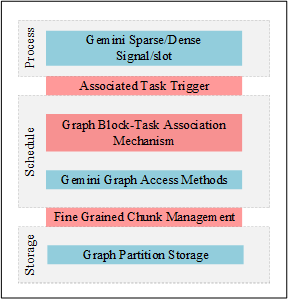
\includegraphics[width=2.5in]{viso插图}
\caption{System Architecture}  
\label{viso插图}
\end{figure}
 
\subsection{Overall Execution Workflow}
We will present the overall execution flow of GraphCPP in pseudo-code. This algorithm takes two input parameters: the set B, containing all graph blocks held by the current computing node, and the set Q, containing all query tasks present on the current computing node. Initially, we allocate a dynamically-sized continuous memory space to store all query tasks (Line 1). Then, we enter a looping process as long as there are unfinished query tasks (Line 2). In this process, GraphCPP calls ChoseNextSharingBlock to update the association between query tasks and graph blocks, and select the currently highest-priority graph block, bi. By calculating the associated blocks for each task (i.e., tasks with active vertices in the current block), we identify all query tasks related to the current graph block bi (Line 4). Next, we load ci into the cache and concurrently process all related query operations, qi (Line 5). We invoke GraphCPPCompute to perform the point-to-point query operation qi on the current block. If the query is not yet complete, we update the state of query qi and generate new query tasks (Line 6). If the newly generated query is associated with the current graph block bi, it is added to Qbi, and we return to Line 5 to continue querying. Otherwise, the information for the newly generated query is stored in the query task collection, and the task is suspended.

\begin{algorithm}
  \caption{Concurrent Point-to-Point Queries on a Set of Graph Blocks Owned by a Graph Partition}
  \label{algorithm:concurrent-queries}
  \begin{algorithmic}[1]
  \Procedure{MallocBuffers}{$B, Q$} \Comment{B is the set of graph blocks, and Q is the set of query tasks}
      \While{\textsc{has\_active}($B$)}
          \State $bi \gets \text{ChooseNextSharingBlock}()$
          \State $Q_{bi} \gets \text{ChooseAssociatedQueries}(bi)$
          \For{$q_i$ \textbf{in} $Q_{bi}$} \Comment{Execute queries in Q in parallel, which is associated with block $bi$}
              \State $new\_query \gets \text{GraphCPPCompute}(q_i, bi)$ \Comment{The implementation function for point-to-point queries returns the active vertex set after one round of task iteration.}
              \If{\textsc{has\_Associated}($(bi, new\_query)$)}
                  \State $Q_{bi}.\text{Push}(new\_query)$
              \Else
                  \State $Q.\text{Push}(new\_query)$
              \EndIf
          \EndFor
      \EndWhile
  \EndProcedure
  \end{algorithmic}
  \end{algorithm}
  
The above algorithm demonstrates the data sharing mechanism in GraphCPP, with the GraphCPPCompute function utilizing the compute sharing mechanism. The following sections will provide a detailed explanation of these two optimization mechanisms.

\subsection{Data Access Sharing Mechanism}
In Section 2.2, we observed a significant overlap in the graph structure data access among concurrent tasks. Under the existing processing mechanism, this overlapping data cannot be shared and utilized. However, for point-to-point query tasks on the graph, the order of data access does not affect the correctness of the results. Our data sharing mechanism essentially transforms the original "task → data" linear task scheduling order into a "data → task" fine-grained concurrent task scheduling order, thereby improving cache utilization efficiency and system throughput. To implement this execution model, we need to address two issues: 1) How to determine the shared data segments? 2) How to implement data sharing among multiple tasks? Below are our implementation details.

A. How to Determine Shared Data Segments?

1.Determine the granularity of shared graph block. Distributed memory graph computing systems need to load data into the cache to improve data access efficiency. Ideally, the data of shared graph should be able to fit entirely into the Last Level Cache (LLC), thereby avoiding the frequent swapping in and out of block parts. However, the granularity of graph blocks should not be too small, as it would increase the synchronization overhead of task processing. We employ formula x to determine an appropriate size for shared graph blocks. In this formula, BS represents the size of the graph structure data for the to-be-determined shared graph block, GS denotes the size of the graph structure data for the partition to which the block belongs, |V| signifies the total number of vertices on the partition, VS stands for the average space needed to store the status information of a vertex, N represents the number of concurrently queried tasks, LLCS denotes the size of the LLC cache space, and RS refers to the reserved redundant space. The two terms on the right side of formula x respectively represent the graph structure data and task-specific data (whose size is proportional to the scale of the graph block and the number of concurrently queried tasks). The right side of the formula indicates the size of the available space for each task after deducting the reserved cache space. Through this formula, we determine the maximum granularity of each shared graph block under the condition of accommodating the LLC capacity.


2. Logical Partitioning. Once the granularity of shared graph blocks is established, GraphCPP can proceed with the logical partitioning during the graph preprocessing phase. This process involves subdividing coarse-grained graph partitions on the distributed system into finer-grained shared graph blocks. Pseudocode for partitioning graph blocks in GraphCPP is presented in Listing X:

\begin{algorithm}
\caption{Logical Partition Algorithm}
\begin{algorithmic}[1]
\Function{Partition}{$P_i, B$} \Comment{B is the set of graph blocks owned by graph partition $P_i$.}
    \State $block\_table \gets$ null
    \For{each $e \in P_i$}  \Comment{$e$ is an edge in partition $P_i$}
        \If{$e.src$ in $block\_table$}
            \State $block\_table[e.src] \mathrel{+{+}}$
        \Else
            \State $block\_table[e.src] \gets 1$
        \EndIf
        \If{$\text{block\_table.size()} \geq SC$}
            \State $B.\text{push}(block\_table)$
            \State $block\_table.\text{clear()}$
        \EndIf
    \EndFor
\EndFunction
\end{algorithmic}
\end{algorithm}

Logical Partitioning Function takes two parameters: one is the graph partition structure data Pi recorded in edge table format, and the other is the and the other is the collection B of graph blocks owned by this partition.   We utilize a dictionary structure called block_table to aggregate information about the graph blocks, where the keys record the source vertex IDs of the edges, and values record the number of outgoing edges for each vertex. Iterate through each edge in the partition. If the edge has already been loaded into the current partition, increment the corresponding count of outgoing edges for that partition. If the vertex is added to the block dictionary for the first time, set the count of outgoing edges for the partition to 1. After processing each edge, check if the current block is full. If so, add the current block to block_set. This way, after traversing all the data in the partition, every edge in the partition is assigned to a specific graph block, resulting in a set of logically partitioned graph blocks.

B. Achieving Data Sharing Among Multiple Tasks

1. Establishing the Association between Shared Blocks and Query Tasks. Through the previous steps, we have achieved fine-grained graph partitioning using a logical approach. Since this is only a logical partitioning, the data remains contiguous on the physical storage medium. Hence, it is easy to determine the partition a vertex belongs to based on its ID. During the execution of a query, each task qi maintains a set of active vertices, Setact,i, following the update policy outlined below:
a. Initially, Set_(act,i) contains only the source vertex Si of the query.

b. The active vertices in Set_(act,i) are processed according to the point-to-point query algorithm, and the processed vertices are removed from the set of active vertices.
c. If a vertex's state is changed in this round and it is not pruned, the vertex is added to Set_(act,i) and awaits processing in the next round.
We first deduce the graph block in which the vertex is located based on its ID, and then use a specially designed array to store the partitions traversed by each task. Since point-to-point queries employ a pruning-based traversal strategy, the number of active vertices in each round is not large. Therefore, it is possible to establish the association between query tasks and their corresponding blocks with relatively low overhead.

2. Determining the Priority of Partition Scheduling. Once the association between query tasks and corresponding blocks is established, we can tally the number of tasks associated with each block. The more tasks associated with a block, the greater the benefits it brings. In this scenario, the block is prioritized for loading into the Last Level Cache (LLC).

3. Triggering Concurrent Execution of Associated Tasks. Having obtained the shared graph data blocks, active query tasks associated with the LLC-resident graph structural data can be deduced. These tasks are executed in batches. As illustrated in Algorithm X, after one round of execution, active tasks generate new active vertices. If these new active vertices are still associated with the current shared block, the query tasks continue execution. The shared block remains in the LLC until all associated query tasks have been processed before it is evicted.

\subsection{Computation Sharing Mechanism}
Tripoline initially introduced the concept of a global index, utilizing idle computational resources to maintain distance values from high-degree vertices to other vertices, thus enabling the sharing of these high-degree vertex distance values across different query tasks. However, the global index mechanism exhibits the following shortcomings:  Shortcoming 1: The global index necessitates the recording of distance values between high-degree vertices and all other vertices. When the graph's scale is extremely large, the computational and storage costs of establishing the index become substantial. Shortcoming 2: In point-to-point queries on streaming graphs, each round of graph updates introduces new edges and edge deletions. The global index requires dynamic updates of the index relationships between high-degree vertices and every vertex based on the latest graph snapshot. This implies that any update to the streaming graph impacts the indexing of all vertices, resulting in a significant computational overhead for maintaining the index.

In general, to better address incoming random queries at any given time, the more high-degree vertices selected, the higher the coverage of overlapping paths, leading to more effective computation sharing. However, as mentioned above, we cannot indefinitely increase the number of high-degree vertices, even if we can allocate a portion of idle computational resources to distribute the costs of calculating and maintaining the index. In response to this, this paper builds upon the global index and introduces a lightweight core subgraph index. Compared to the global index, the core subgraph index has a smaller selection threshold and a higher quantity of high-degree vertices, enabling a higher coverage and providing more precise upper bound values. Additionally, it no longer maintains distance values from high-degree vertices to all vertices; instead, it only needs to maintain indices among high-degree vertices. Consequently, its overhead is significantly reduced compared to the global index. Pseudocode for core subgraph query is shown in Listing XXXX.

\begin{algorithm}
    \caption{Core Subgraph Query Algorithm}
    \begin{algorithmic}[1]
    \State $global\_index \gets \text{BuildGlobalIndex}(k)$ \Comment{Step 1: Calculate $k$ Global Index}
    \State $core\_subgraph\_index \gets \text{BuildCoreSubgraphIndex}(m, global\_index)$ \Comment{Build $m$ Core Subgraph Index}
    \Function{GraphCPPCompute}{$q, b$}
        \State $active\_vertices \gets \text{InitializeActiveVertices}(q, b)$ \Comment{Determine active vertices based on query task and graph block}
        \State \Call{InitializeBoundsFromGlobalIndex}{$global\_index$} \Comment{Initialize bounds based on the global index}
        \While{$\text{active\_vertices is not empty}$}
            \For{$vertex$ in $active\_vertices$}
                \If{$vertex$ is in $core\_subgraph$}
                    \State \Call{UpdateBoundsByCoreVertices}{$vertex, core\_subgraph\_index$}
                \Else
                    \For{$nbr$ in \Call{GetOutgoingNeighbors}{$vertex$}} \Comment{Traverse outgoing neighbors of $vertex$}
                        \State \Call{UpdateBoundsByNeighbors}{$nbr$}
                    \EndFor
                \EndIf
            \EndFor
            \State $active\_vertices \gets \text{UpdateActiveVertices}()$
        \EndWhile
    \EndFunction
    \end{algorithmic}
    \end{algorithm}


The execution steps for achieving computation sharing are as follows: 1. Establish a Global Index (Lines 1): We employ a strategy similar to SGraph for computing the global index. After sorting the degrees of vertices, the system selects the top k vertices with the highest degrees (where the value of k is user-determined). Subsequently, an SSSP algorithm is executed to compute the shortest paths (including distance values and path parent nodes) between these k high-degree vertices and all vertices in the graph. The results are stored in an array indexed by the IDs of the high-degree vertices. 2. Establish a Core Subgraph Index (Lines 2): Allowing more high-degree vertices, typically one order of magnitude larger than k, which are ranked in the top m in terms of degree, to be included in the core subgraph. As the global index vertices have already recorded the indices to reach the global index, these vertices are excluded. Additionally, once the global index is established, point-to-point queries for the shortest paths between points on the core subgraph can be directly computed using upper and lower bound pruning. 3. Query Acceleration (Lines 3): Perform point-to-point queries, starting by utilizing the global index to determine approximate upper and lower bounds. Subsequently, pruning queries begin. Under normal circumstances, the system traverses each outgoing edge vertex of the current vertex, sequentially performing pruning checks on the distance values of each vertex to determine the next round of active vertices. If the current query vertex belongs to the core subgraph, in addition to visiting neighboring out-edge vertices, all other high-degree vertices connected to this vertex must also be accessed. Under normal circumstances, the state propagation between these high-degree vertices may require multiple hops. With the core subgraph, the propagation between these points can be accomplished in a single step. In addition to expediting state propagation, a hidden factor is that the core subgraph is populated with high-degree vertices, making them more likely to appear on the shortest path between two points, thereby expediting the path discovery process. 4. Query Termination (Lines 6): Apply upper and lower bound query techniques for pruning. For unidirectional queries, starting from the source vertex, reaching the destination vertex indicates the discovery of a path. For bidirectional queries, the convergence of queries from both directions indicates the discovery of a path. If a new path value is smaller than the current upper bound, it is updated as the new upper bound. If the path value is greater than the current upper bound, it is pruned. The discovery of a path does not imply the end of iteration; it is necessary to assess the active vertices in the graph. Only when all possible paths have been attempted, the upper bound is updated to the shortest path value, and all vertex edge path values are greater than the current upper bound, and the number of active vertices decreases to zero, does the iteration conclude. Through the aforementioned steps, we achieve efficient data sharing using the lightweight core subgraph index.

\subsection{Other Optimization}
1. Core Subgraph Maintenance:

GraphCPP streamlines the traditional "global index," which maintains distance values for all vertices, into a "core subgraph index" that only maintains distance values between high-degree vertices. During computation, the global index is reused to perform point-to-point queries based on upper and lower bound pruning to obtain the shortest path values between high-degree vertices on the core subgraph. In terms of storage, each high-degree vertex only needs to store a small amount of distance values between high-degree vertices. Clearly, compared to the global index, both the computational and storage costs of the core subgraph index are significantly reduced. Additionally, for index maintenance on dynamic graphs, we have implemented special optimizations. Specifically, when calculating the shortest path between high-degree vertices, each vertex records its parent node on the path. When the final path converges, we can obtain the set of all vertices on the shortest path by retracing from the destination vertex. We store each set of shortest paths indexed by the starting point of the path. When a graph update occurs, we first check whether the affected active vertices are part of any shortest path. If they are not, the index remains unaffected and does not require an update. If they are, we need to recalculate the distance values for that index.

2. Batch Execution of Similar Tasks

Different query tasks arrive randomly, and they often follow distinct traversal paths. We observed that when two tasks have very low similarity, their overlapping path proportion decreases, and there might be no overlap at all. However, if the starting and target vertices of two queries are located in adjacent data blocks within the graph, the paths they traverse during the query process are highly likely to be close to each other. To address this, we propose a strategy for batch executing similar tasks, selecting batches of similar tasks from the task pool at a time to further leverage data similarity.Specifically, GraphCPP first randomly selects a query task from the task pool, obtaining the starting and target vertices of the task. It then executes a k-hop SSSP to retrieve the neighboring vertex sets SetS for the starting vertex and SetD for the target vertex (the value of k is determined by the user and is typically set to 3 by default). Subsequently, it iterates through the task pool, filtering out all the query tasks where the starting point is in SetS and the target point is in SetD. These tasks are treated as similar tasks and executed concurrently.It is worth noting that if the starting or target vertex of a query belongs to a high-degree vertex, the index can be directly used to accelerate the query process, bypassing the regular query steps. Excluding the high-degree vertices, the overhead of the k-hop SSSP is minimal, and the execution can be done concurrently with normal queries, with negligible additional costs.

\section{EXPERIMENTAL EVALUATION}

\section{RELATED WORK}
Point-to-Point Queries: Existing work has conducted extensive research on point-to-point queries. For instance, 𝐻𝑢𝑏2 [x] proposed a hub-centric specialized accelerator, which contends that vertices with a large number of connections, i.e., hubs, expand the search space, making shortest path calculations exceptionally challenging. It introduced the hub-Network concept to confine the search scope of hub nodes. The online pruning of hub search process was achieved using the hub2-Labeling method. However, due to 𝐻𝑢𝑏2's specialization in a dedicated accelerator, its applicability is limited. PnP observed the traversal process of point-to-point queries and introduced an upper-bound-based pruning strategy, reducing unnecessary vertex traversals and providing a fresh perspective for point-to-point query research. Tripoline derived an approximate "upper bound" between two points by maintaining some "permanent vertices" in daily operations, using them as intermediaries. This approach enabled "prior-knowledge-free" upper bound queries. SGraph further developed on the aforementioned methods, leveraging the triangle inequality principle on the graph to propose upper-bound and lower-bound pruning strategies, achieving sub-second point-to-point queries on the graph. However, these systems mainly focus on optimizing the speed of individual point-to-point queries, overlooking the severe load of large-scale concurrent queries.

Concurrent Graph Computing: Numerous graph computing systems have explored concurrent computing. GraphM pointed out the "data access similarity" among concurrent graph computing tasks and proposed a data-centric scheduling strategy to facilitate data sharing between multiple tasks, thereby enhancing the throughput of concurrent graph computing. However, GraphM is a single-machine out-of-core graph computing system that adopts the BSP computing model and is only applicable to static graphs. Building upon this, CGraph[x] extended the application scenarios to distributed dynamic graph computing systems. It optimized the communication mechanism and load balancing strategy for distributed scenarios. However, like GraphM, it is still an out-of-core system and is not suitable for high-load scenarios of concurrent queries, even though it can distribute the disk access cost across different subgraphs through scheduling strategies. ForkGraph efficiently conducts concurrent graph processing in memory and employs a concession-based scheduling strategy, handling only a portion of the data in each iteration to accelerate overall execution speed. However, it is a single-machine in-memory system and has not been optimized for point-to-point queries, making it unsuitable for executing concurrent point-to-point query tasks on massive datasets.

\section{CONCLUSION}
This paper introduces a concurrent point-to-point query system, GraphCPP, which leverages data similarity between concurrent queries to achieve data sharing among multiple tasks. Furthermore, it employs a lightweight core subgraph index to enhance computation sharing among multiple tasks. Experimental results demonstrate that GraphCPP outperforms the state-of-the-art graph query system, SGraph, by a factor of XXX.

\section{ACKNOWLEDGMENTS}


\begin{thebibliography}{1} %这里的1是指用最多的数字有几位,比如10就是指用最多的数字有两位

\bibitem{ams} %这行是指把这个参考文献标签为ams,这个标签可以自己取,作用是在正文中引用时用的
{\it{Mathematics into Type}}, American Mathematical Society. Online available:  %\it的意思是把后面的内容变成斜体

\bibitem{oxford} %这行是指把这个参考文献标签为oxford
T.W. Chaundy, P.R. Barrett and C. Batey, {\it{The Printing of Mathematics}}, Oxford University Press. London, 1954.

\bibitem{lacomp}{\it{The \LaTeX Companion}}, by F. Mittelbach and M. Goossens

\bibitem{mmt}{\it{More Math into LaTeX}}, by G. Gr\"atzer

\bibitem{amstyle}{\it{AMS-StyleGuide-online.pdf,}} published by the American Mathematical Society

\bibitem{Sira3}
H. Sira-Ramirez. ``On the sliding mode control of nonlinear systems,'' \textit{Systems \& Control Letters}, vol. 19, pp. 303--312, 1992.

\bibitem{Levant}
A. Levant. ``Exact differentiation of signals with unbounded higher derivatives,''  in \textit{Proceedings of the 45th IEEE Conference on Decision and Control}, San Diego, California, USA, pp. 5585--5590, 2006.

\bibitem{Cedric}
M. Fliess, C. Join, and H. Sira-Ramirez. ``Non-linear estimation is easy,'' \textit{International Journal of Modelling, Identification and Control}, vol. 4, no. 1, pp. 12--27, 2008.

\bibitem{Ortega}
R. Ortega, A. Astolfi, G. Bastin, and H. Rodriguez. ``Stabilization of food-chain systems using a port-controlled Hamiltonian description,'' in \textit{Proceedings of the American Control Conference}, Chicago, Illinois, USA, pp. 2245--2249, 2000. %这里的\textit是指把后面的内容变成斜体

\end{thebibliography} %这个是参考文献的结束

\begin{IEEEbiographynophoto}{Jane Doe} %这里的Jane Doe是指作者的名字
Biography text here without a photo.
\end{IEEEbiographynophoto} %这个是作者的结束

\begin{IEEEbiography}[{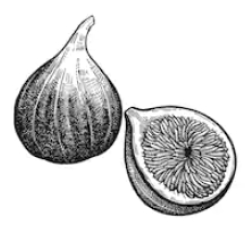
\includegraphics[width=1in,height=1.25in,clip,keepaspectratio]{fig1.png}}]{IEEE Publications Technology Team}
In this paragraph you can place your educational, professional background and research and other interests.\end{IEEEbiography} %这行的作用是插入作者的照片


\end{document}


